\documentclass{article}
\usepackage{fontspec} % Load fontspec first
\usepackage{microtype} % for better typography
\usepackage{graphicx}
\usepackage{float}
\usepackage{subfiles}
\usepackage{ragged2e}
\usepackage{geometry}

\graphicspath{{./}}
% Additional packages and configurations


% Set the font to a serif font (Times New Roman)


% Set title spacing to 0
\usepackage{titling} % for title spacing control
\setlength{\droptitle}{-10em} 
\linespread{1.1} % adjust line spacing
% Set wider margins
\geometry{
    left=4cm,
    right=4cm,
    top=3cm,
    bottom=3cm,
}






\begin{document}
\title{Operational NMOS amplifier with NMOS differential pair}
\author{Vasco Luz} % Fill in your name
\date{2024-02-13} % Set the date
\maketitle
\justify

\section{Intruduction}


Automatic generated report in order to showcase this amplifier characteristics.
\newline
This is a low power 5V 5 transistor OTA with an NMOS amplifier.
\newline
The amplifier instance os called 5V low power 5trans NMOS amplifier.
\newline
By changing the reference current, it will have different characteristics.

\section{Current bias generation Characterization}

Characterization of the current bias generation.
\newline
Fig.\ref{fig:values} represents the minimum voltage allowed for the current reference to work.
\begin{figure}[H] % Use H option for float placement
    \centering
    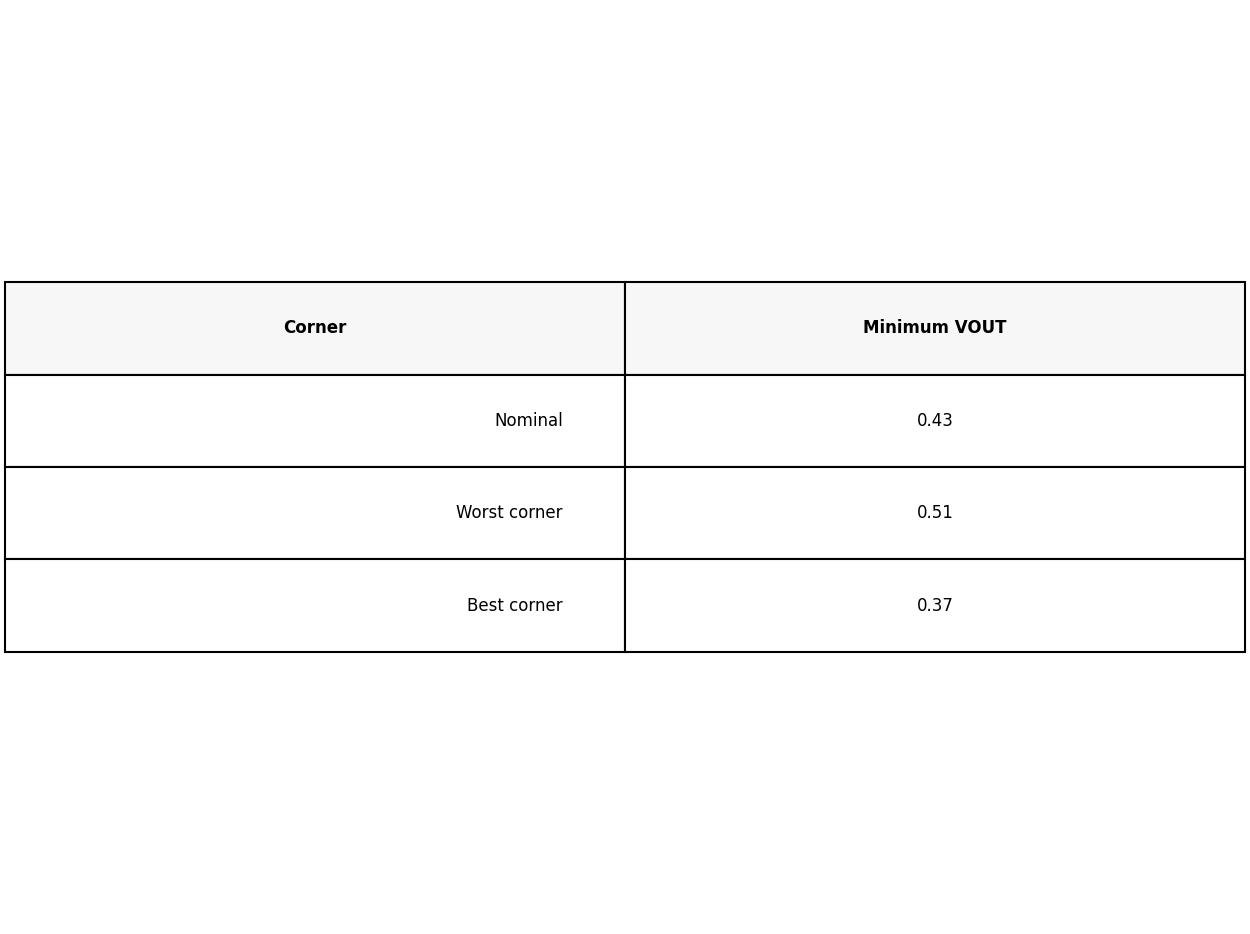
\includegraphics[width=.6\textwidth]{./interception_table.jpg} % Assuming this is the image generated by your Python script
    \caption{minimum voltage}\label{fig:values}
\end{figure}



Fig.\ref{fig:iout_vs_vout} represent the output current characteristic for nominal, worst and best case scenario.

\begin{figure}[H] % Use H option for float placement
    \centering
    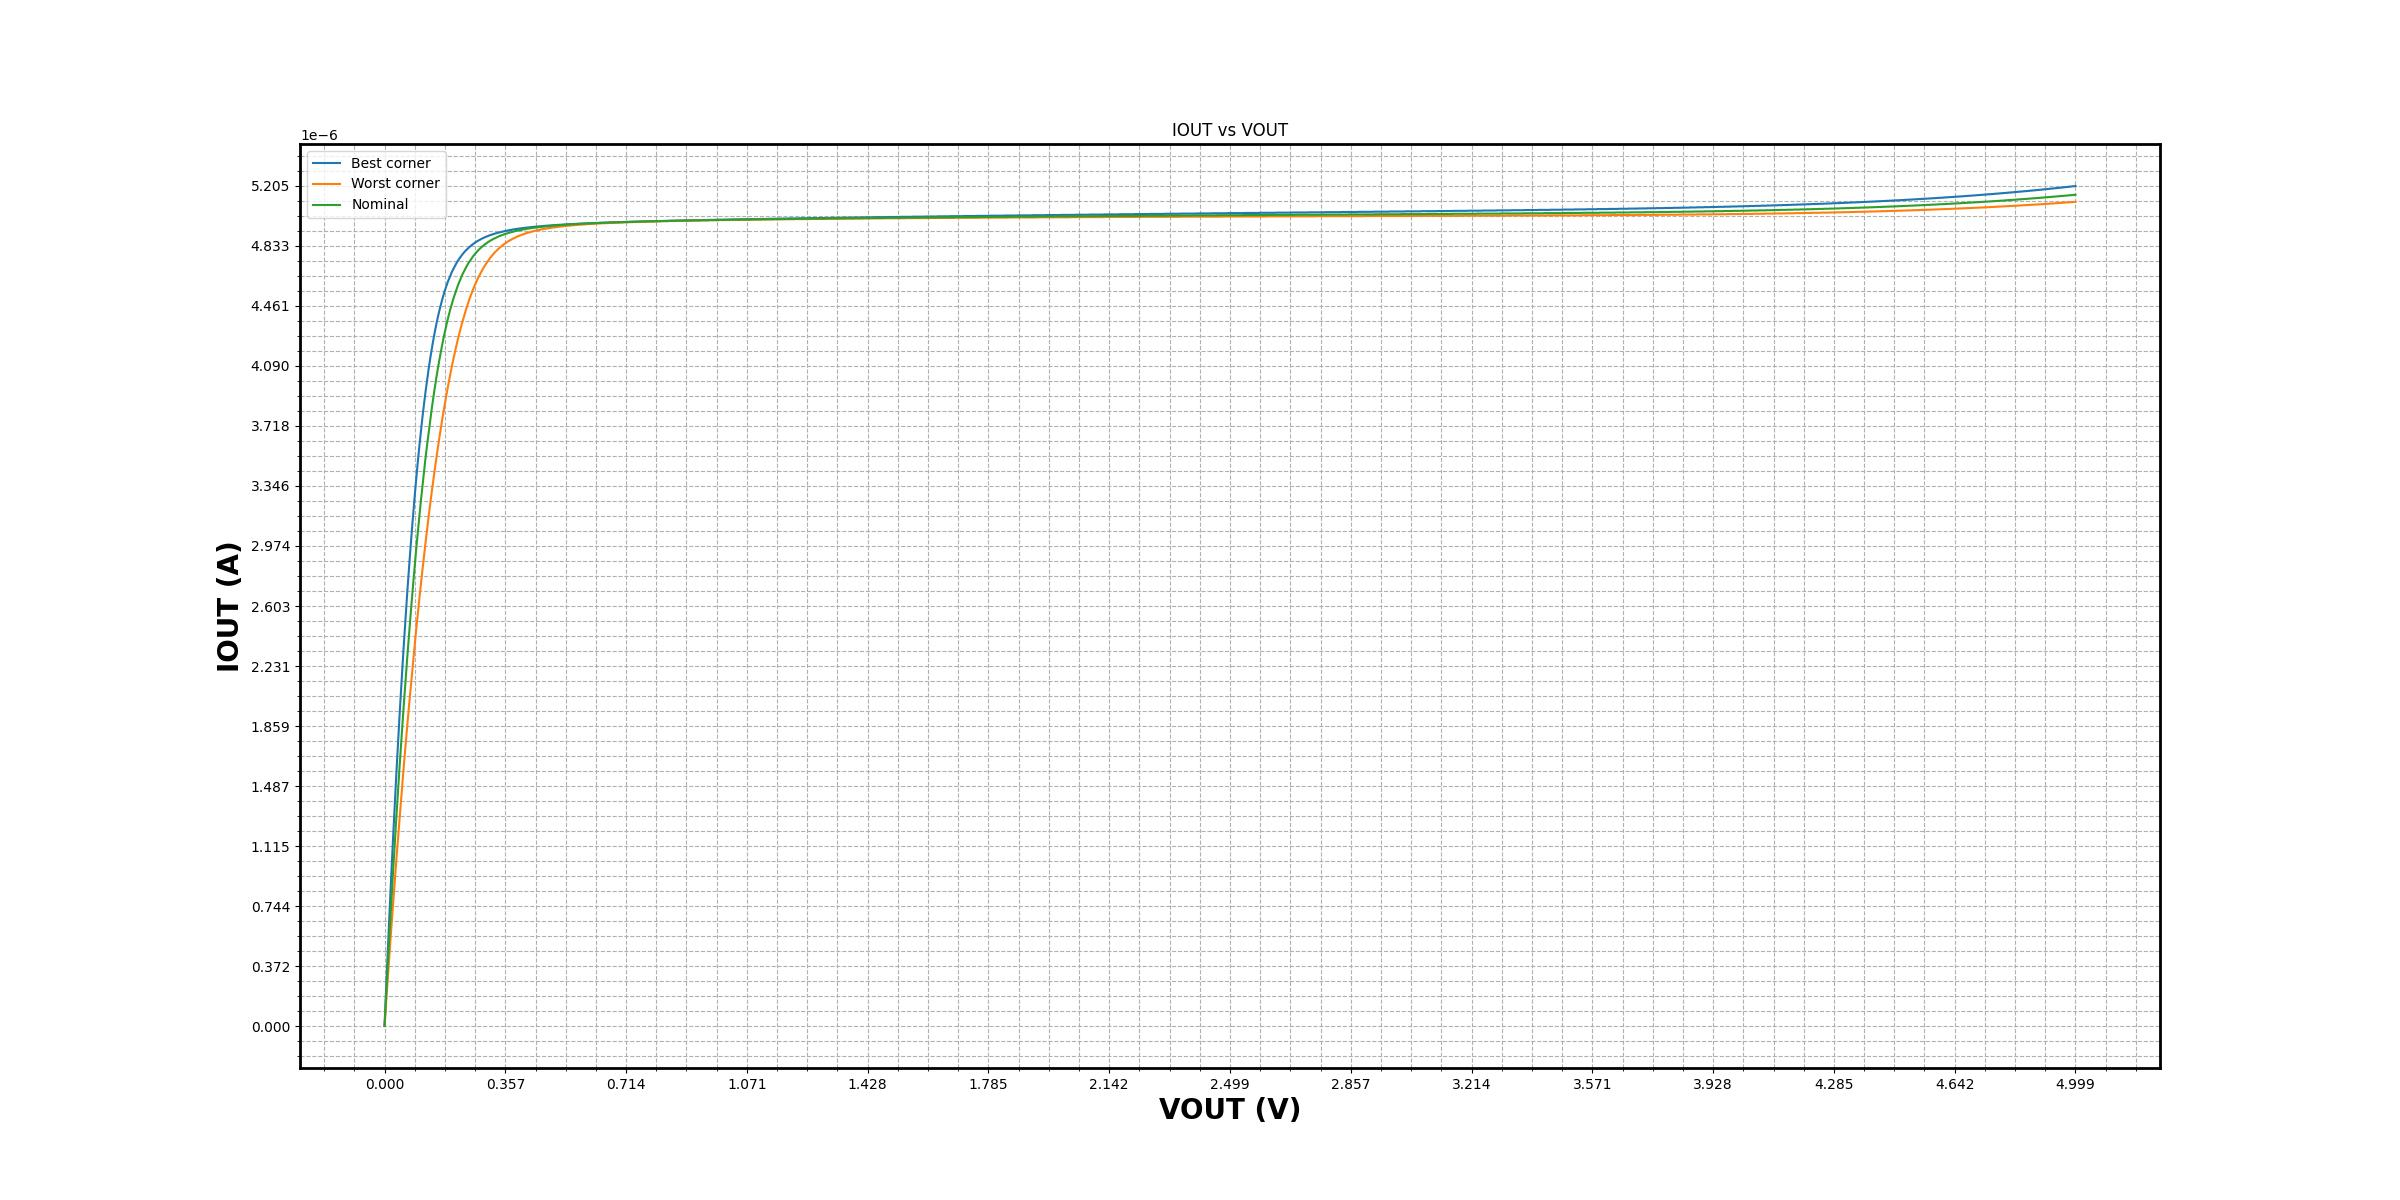
\includegraphics[width=.6\textwidth]{./IOUT_vs_VOUT.jpg} % Assuming this is the image generated by your Python script
    \caption{IOUT vs VOUT}\label{fig:iout_vs_vout}
\end{figure}




Fig.\ref{fig:output_impedance} represent the output impedance characteristic for nominal, worst and best case scenario.

\begin{figure}[H] % Use H option for float placement
    \centering
    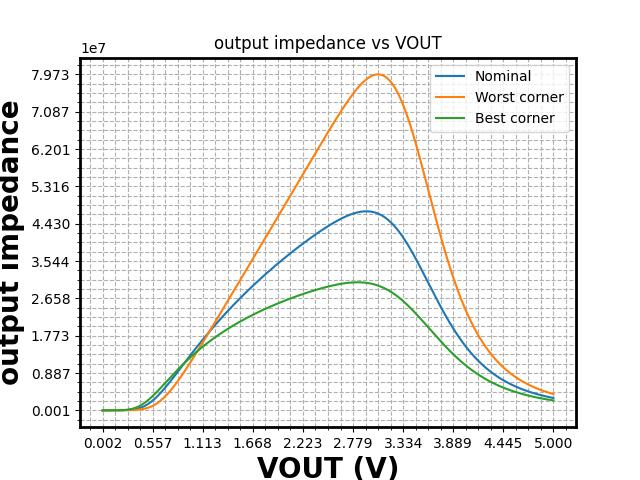
\includegraphics[width=.6\textwidth]{./output_impedance_vs_VOUT.jpg} % Assuming this is the image generated by your Python script
    \caption{output impedance}\label{fig:output_impedance}
\end{figure}



Fig.\ref{fig:ac_current_variation} represent the current variation face an ac signal for nominal, worst and best case scenario.

\begin{figure}[H] % Use H option for float placement
    \centering
    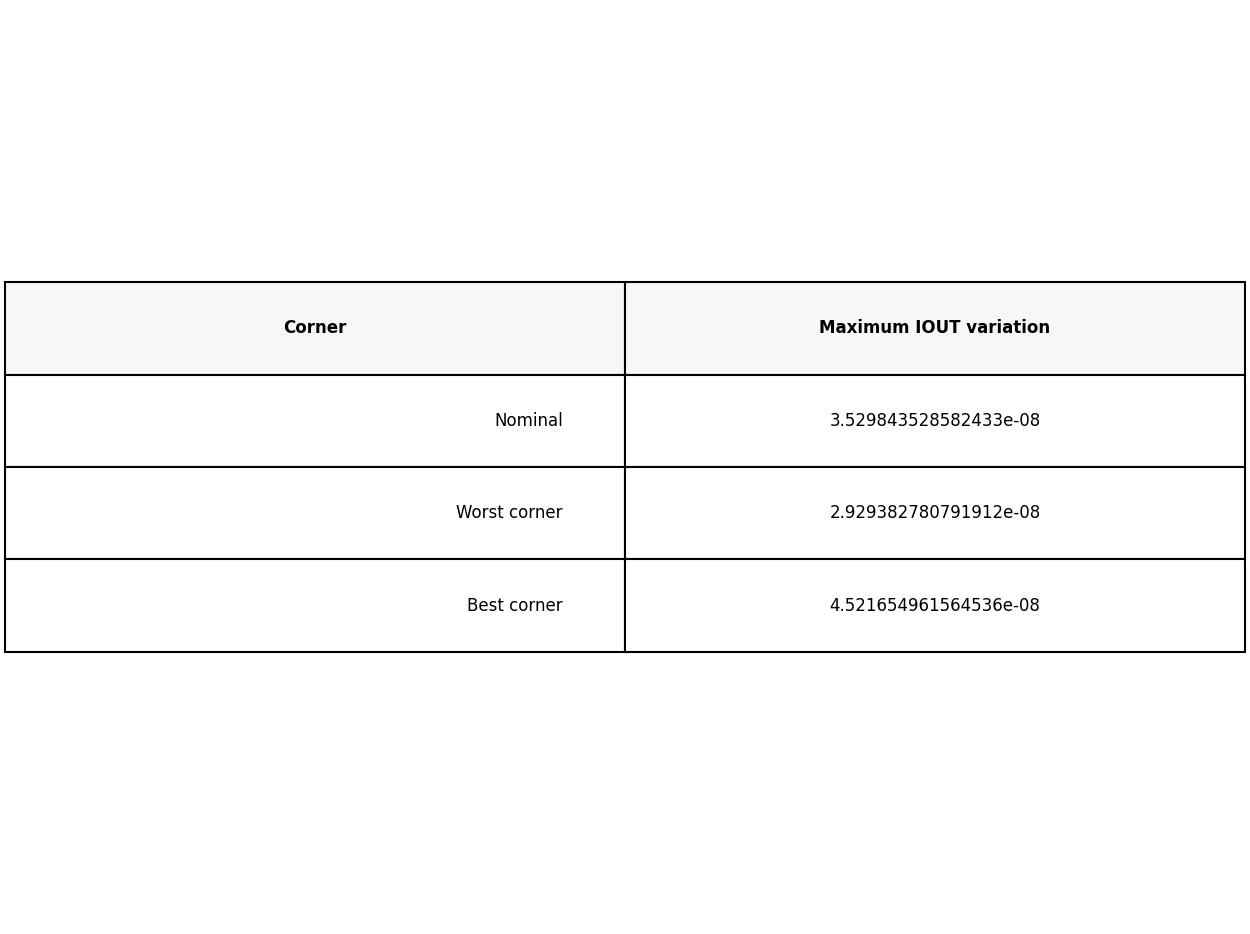
\includegraphics[width=.6\textwidth]{./ac_bias_table.jpg} % Assuming this is the image generated by your Python script
    \caption{ac variation}\label{fig:ac_current_variation}
\end{figure}

Fig.\ref{fig:nominal} represent the current variation at vout = VDD/2 with 200 runs.

\begin{figure}[H] % Use H option for float placement
    \centering
    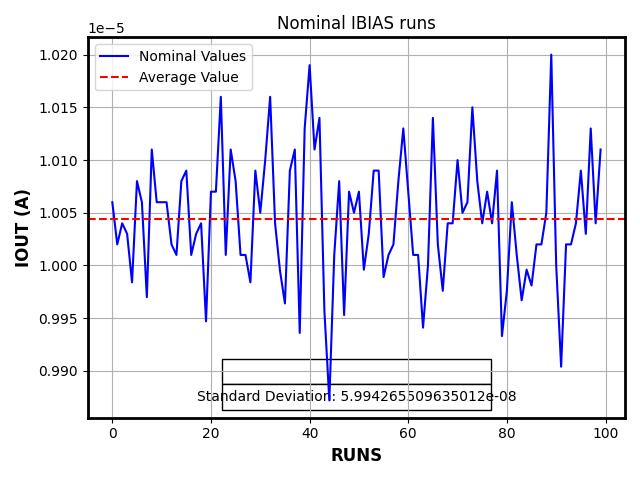
\includegraphics[width=.6\textwidth]{./Nominal_IBIAS_runs.jpg} % Assuming this is the image generated by your Python script
    \caption{Monte carclo variations}\label{fig:nominal}
\end{figure}


Fig.\ref{fig:histogram} represent the histogram.

\begin{figure}[H] % Use H option for float placement
    \centering
    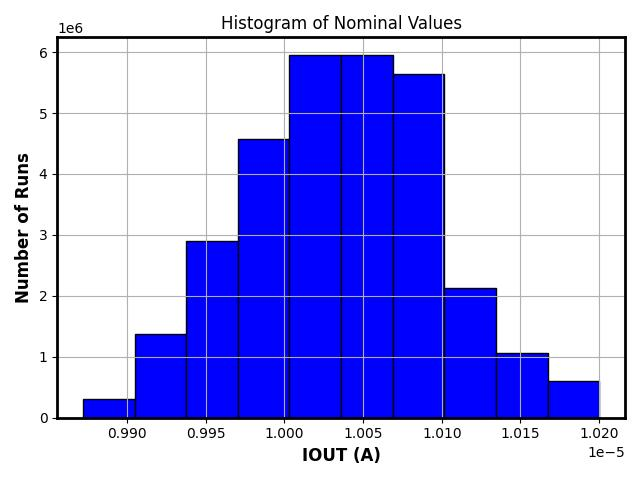
\includegraphics[width=.6\textwidth]{./Nominal_IBIAS_runs_histogram.jpg} % Assuming this is the image generated by your Python script
    \caption{Monte carclo variations}\label{fig:histogram}
\end{figure}


\section{PMOS load characteristics}

It is the relation of VOUT and temperature. Its important to note that the load was sized so when the current is equal in each size $V_{OUT} = V_{DD}/2$
\newline






Fig.\ref{fig:load_characteristic} is the most important load characteristic. Its basicly the relation between the current and VOUT. Its important in order to define the VOUT DC and the effective swing.
\newline
This characteristic is used so the user can adapt to diferent scenarios with the a change of IREF.


\begin{figure}[H] % Use H option for float placement
    \centering
    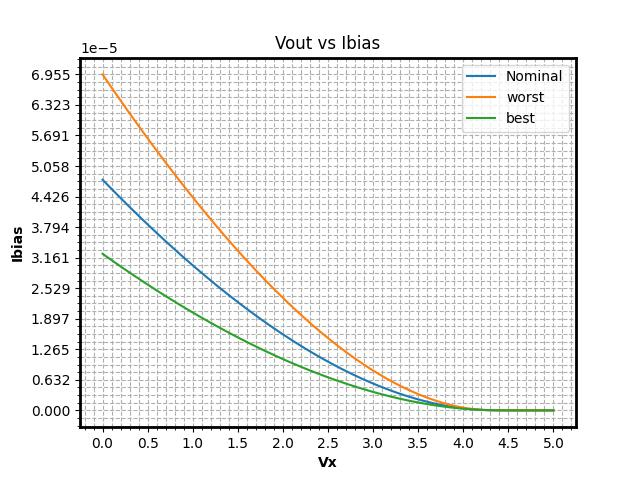
\includegraphics[width=.6\textwidth]{./only_PMOS_LOAD_current_characteristic.jpg} % Assuming this is the image generated by your Python script
    \caption{Load current characteristic}\label{fig:load_characteristic}
\end{figure}











Load impedance with the bias generator, determines the dc value of $V_{OUT}$, to this case we center its value to $V_{DD}/2$ at 27 degrees at tt corner. Fig.\ref{fig:table_vout} shows the dispersion of VOUT at the worst corners.
\begin{figure}[H] % Use H option for float placement
    \centering
    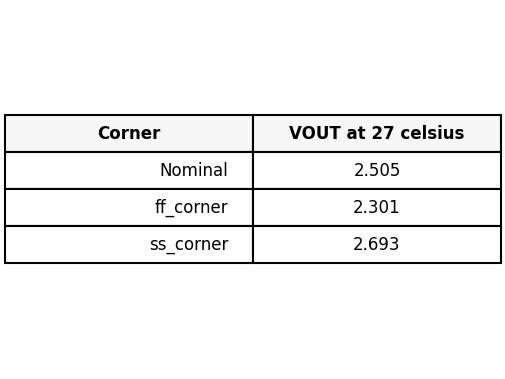
\includegraphics[width=.6\textwidth]{./only_PMOS_LOAD_VDC_NMOS_table.jpg} % Assuming this is the image generated by your Python script
    \caption{VOUT defenition in fucntion of the load}\label{fig:table_vout}
\end{figure}

Fig.\ref{fig:vout_temp_var}  shows the variation of VOUT in fucntion of temperature.

\begin{figure}[H] % Use H option for float placement
    \centering
    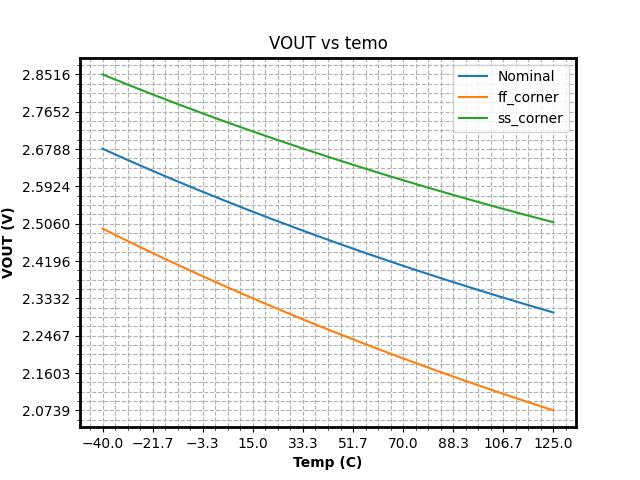
\includegraphics[width=.6\textwidth]{./only_PMOS_LOAD_VDC_NMOS.jpg} % Assuming this is the image generated by your Python script
    \caption{VOUT defenition in function of the temperature}\label{fig:vout_temp_var}
\end{figure}




Fig.\ref{fig:vout_temp_var_monte}  shows the variation of VOUT in fucntion of a monte carlo simulation.

\begin{figure}[H] % Use H option for float placement
    \centering
    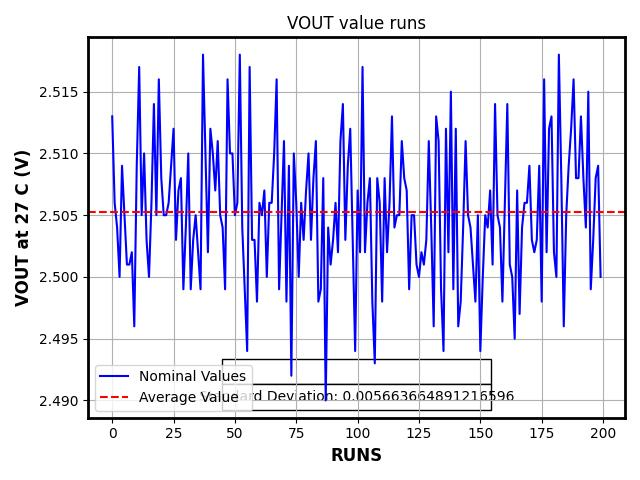
\includegraphics[width=.6\textwidth]{./VOUT_value_runs.jpg} % Assuming this is the image generated by your Python script
    \caption{VOUT vs monte carlo}\label{fig:vout_temp_var_monte}
\end{figure}




Fig.\ref{fig:vout_temp_var_hist}  shows the variation of VOUT in fucntion of a monte carlo simulation in histogram form.

\begin{figure}[H] % Use H option for float placement
    \centering
    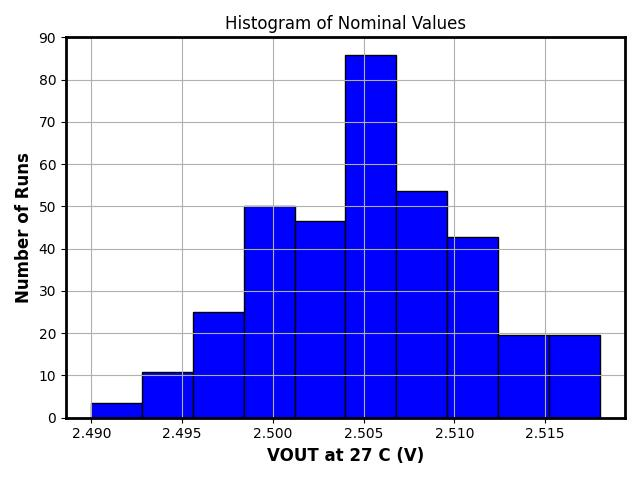
\includegraphics[width=.6\textwidth]{./VOUT_value_runs_histogram.jpg} % Assuming this is the image generated by your Python script
    \caption{VOUT vs monte carlo histogram}\label{fig:vout_temp_var_hist}
\end{figure}





\section{Differential pair characteristics}

Fig.\ref{fig:_input_table}, represents the minimum allowed input voltage for the differential pair.  This analysis is based on the current.

\begin{figure}[H] % Use H option for float placement
    \centering
    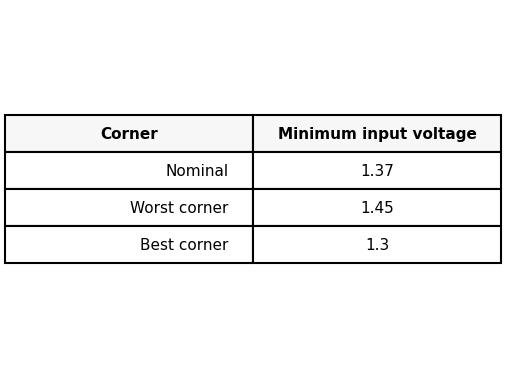
\includegraphics[width=.6\textwidth]{./Minimum_input_voltage_table.jpg} % Assuming this is the image generated by your Python script
    \caption{Minimum input voltage table}\label{fig:_input_table}
\end{figure}



Fig.\ref{fig:_input_pair}, differential pair current characteristic.

\begin{figure}[H] % Use H option for float placement
    \centering
    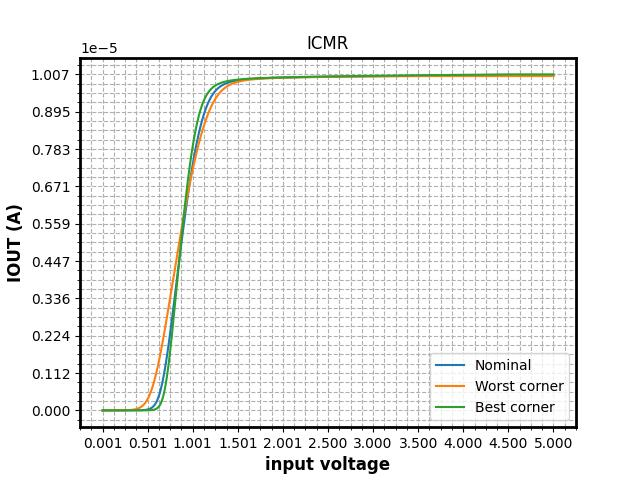
\includegraphics[width=.6\textwidth]{./Minimum_input_voltage.jpg} % Assuming this is the image generated by your Python script
    \caption{Minimum input voltage table}\label{fig:_input_pair}
\end{figure}




\end{document}